\begin{figure}[t]
\centerline{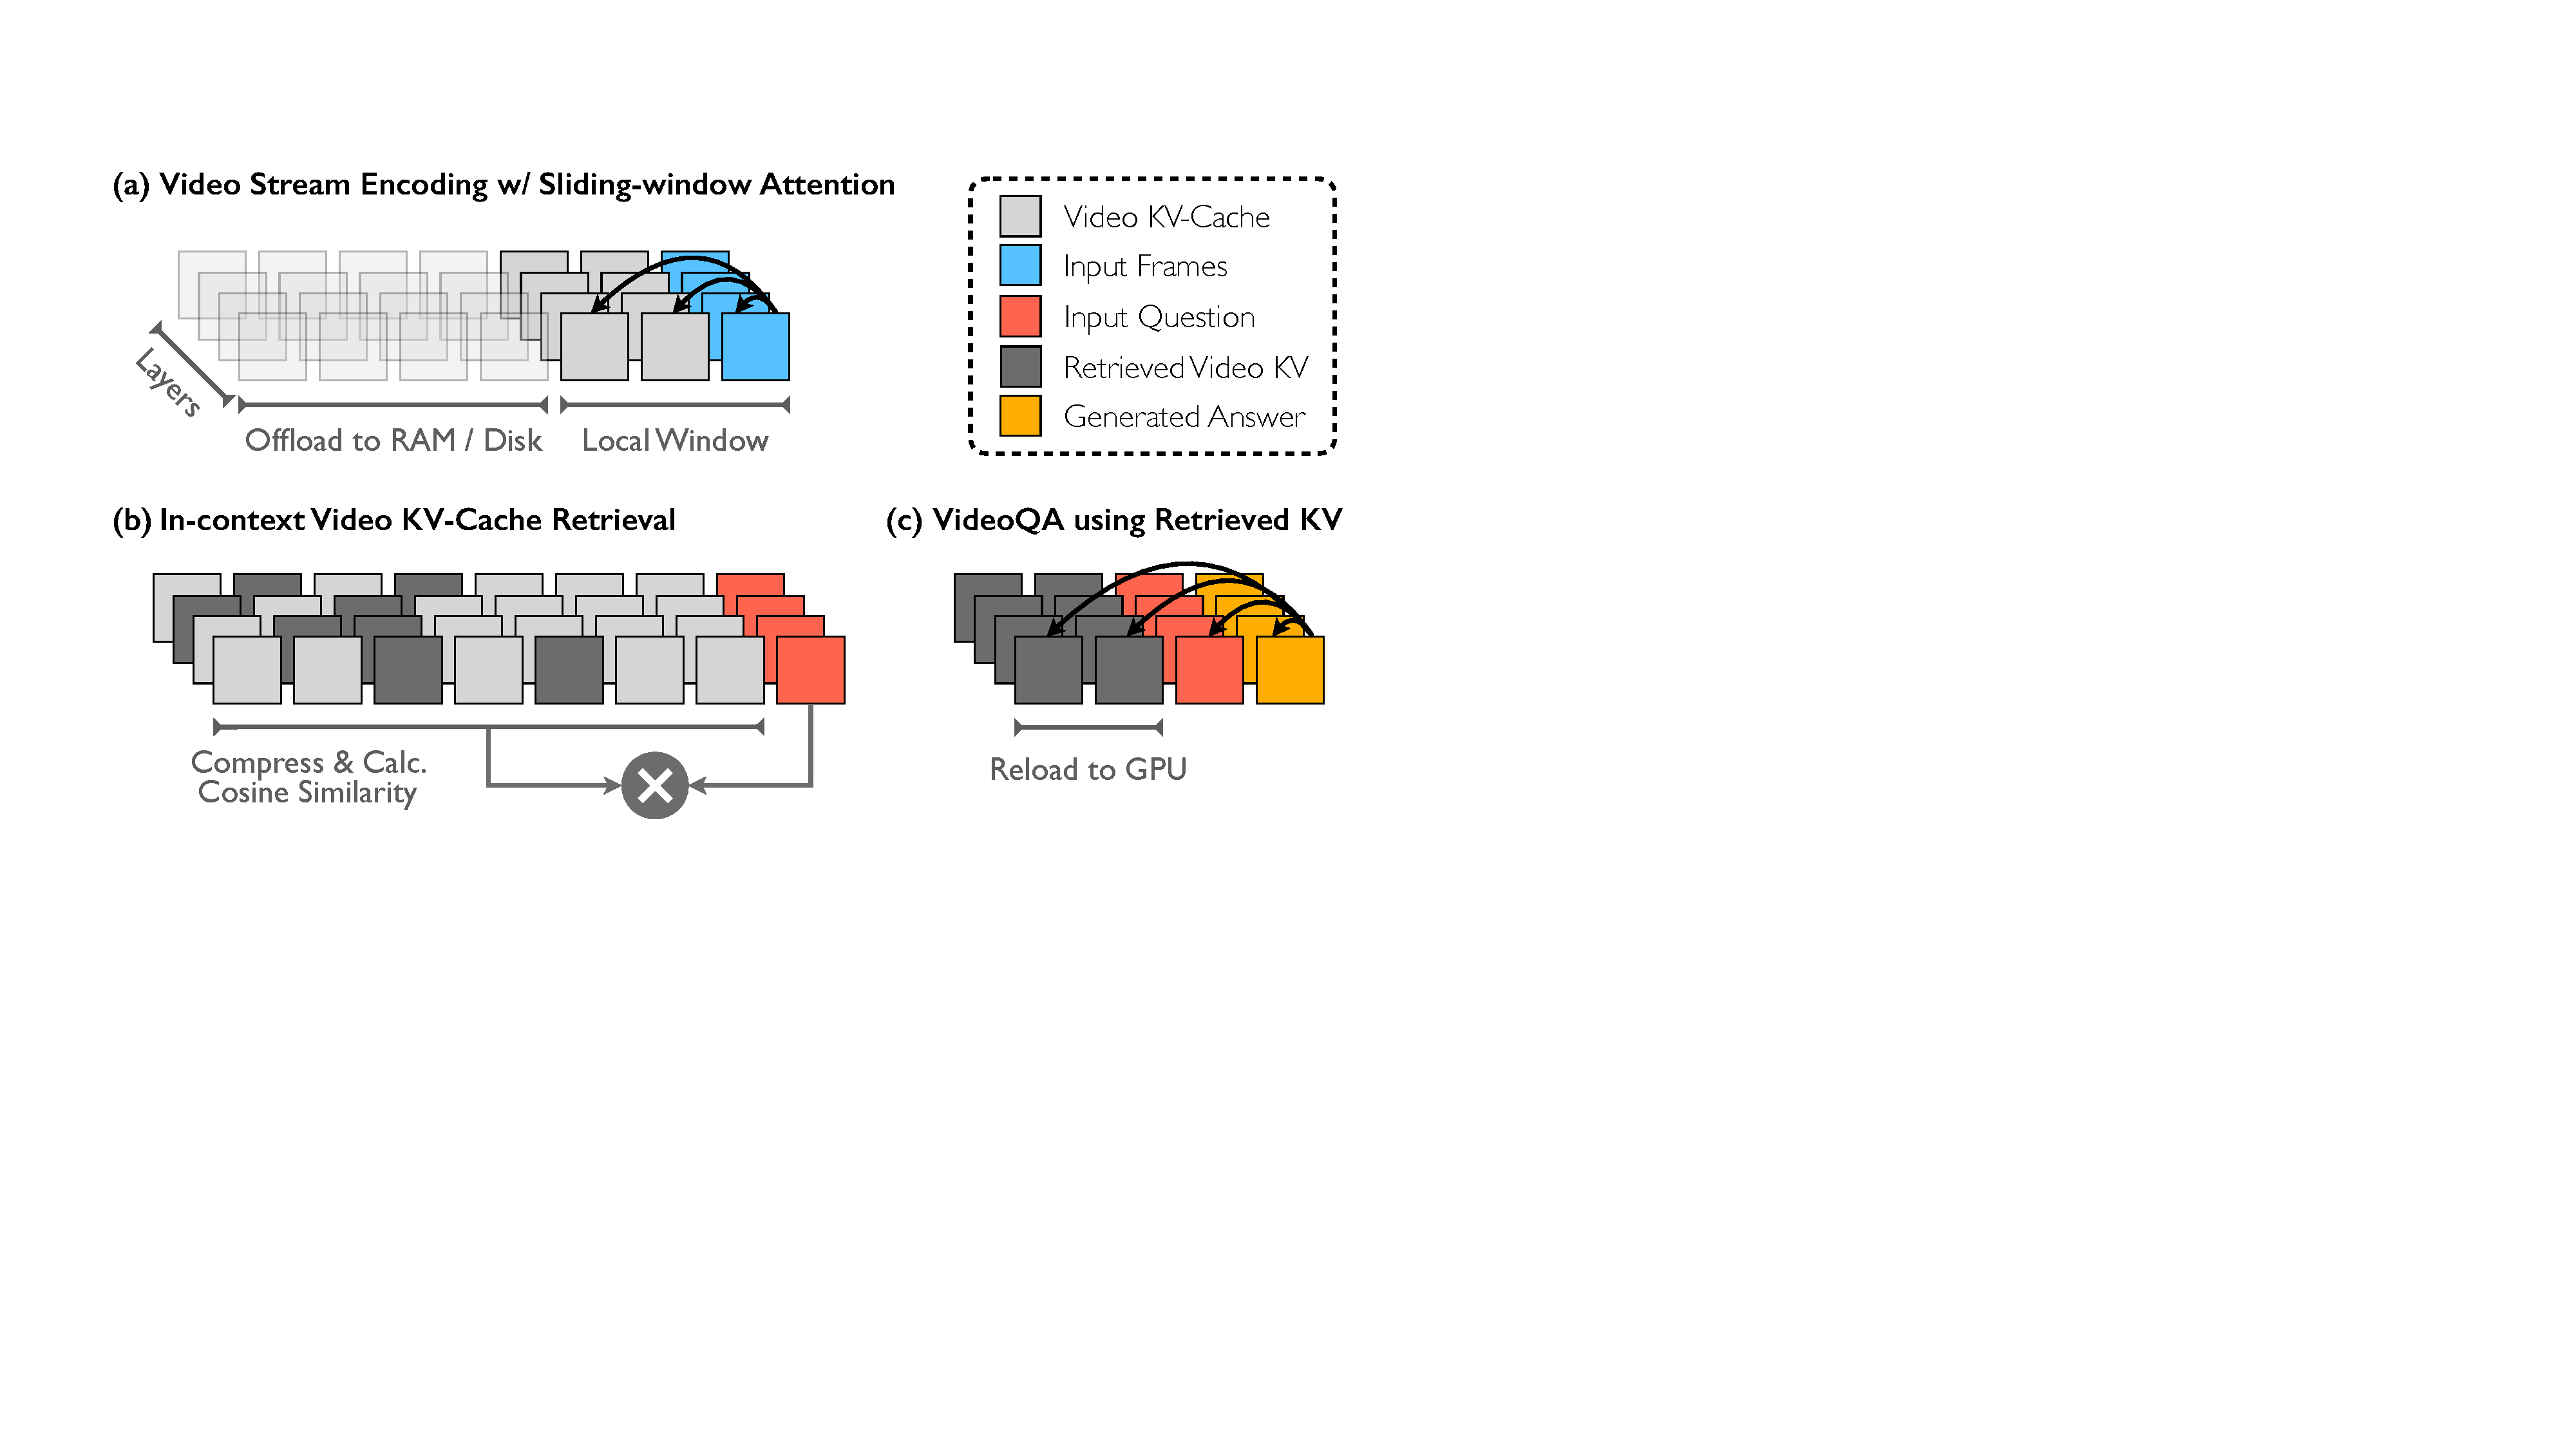
\includegraphics[width=.85\linewidth]{figures/src/framework.pdf}}
\caption{
\textbf{Descripción general de~\ourmethod.}
Modificamos el mecanismo de atención en los Video-LLMs basados en decoder:
(a) el flujo de video se codifica con atención de ventana deslizante (Ecuación~\ref{equ:video_encoding}), con las Video KV-Caches fuera de la ventana descargadas a RAM o disco.
(b) al recibir una pregunta, se recuperan key-value vectors relevantes en función de la similitud coseno, con vectores comprimidos para acelerar el retrieval (Ecuación~\ref{equ:retrieval}).
(c) los key-value vectors recuperados se recargan en la GPU y se utilizan para la generación autoregresiva de respuestas (Ecuación~\ref{equ:answer_generation}).
}
\label{fig:framework} 
\end{figure}
